\documentclass[12pt,a4paper]{article}

% Required packages
\usepackage[utf8]{inputenc}
\usepackage[T1]{fontenc}
\usepackage{graphicx}
\usepackage{amsmath}
\usepackage{amssymb}
\usepackage[hidelinks]{hyperref}
\usepackage{geometry}
\geometry{margin=1in}
\usepackage{xcolor}
\usepackage{tcolorbox}
\usepackage{titlesec}
\usepackage{enumitem}
\usepackage{tikz}

% Define colors for backgrounds - subtle and professional
\definecolor{theoremblue}{RGB}{230,245,255}
\definecolor{formulayellow}{RGB}{255,252,235}
\definecolor{definitiongreen}{RGB}{240,255,245}
\definecolor{importantpink}{RGB}{255,240,248}

% Custom boxes for important content - subtle colors
\newtcolorbox{theorembox}{
  colback=theoremblue,
  colframe=blue!40!black,
  boxrule=0.5pt,
  arc=2mm,
  left=5pt,
  right=5pt,
  top=5pt,
  bottom=5pt
}

\newtcolorbox{formulabox}{
  colback=formulayellow,
  colframe=orange!40!black,
  boxrule=0.5pt,
  arc=2mm,
  left=5pt,
  right=5pt,
  top=5pt,
  bottom=5pt
}

\newtcolorbox{definitionbox}{
  colback=definitiongreen,
  colframe=green!35!black,
  boxrule=0.5pt,
  arc=2mm,
  left=5pt,
  right=5pt,
  top=5pt,
  bottom=5pt
}

\newtcolorbox{importantbox}{
  colback=importantpink,
  colframe=red!30!black,
  boxrule=0.5pt,
  arc=2mm,
  left=5pt,
  right=5pt,
  top=5pt,
  bottom=5pt
}

% Customize section headings
\titleformat{\section}
  {\normalfont\Large\bfseries}{\thesection}{1em}{}
\titleformat{\subsection}
  {\normalfont\large\bfseries}{\thesubsection}{1em}{}
\titleformat{\subsubsection}
  {\normalfont\normalsize\bfseries}{\thesubsubsection}{1em}{}

% Define tightlist command for compatibility
\providecommand{\tightlist}{%
  \setlength{\itemsep}{0pt}\setlength{\parskip}{0pt}}

\begin{document}

% Suppress page numbering for the first 3 pages
\pagenumbering{gobble}

% ============================================
% PAGE 1 - TITLE PAGE
% ============================================
\thispagestyle{empty}
\begin{center}

\vspace*{2cm}

{\fontsize{16}{19}\selectfont \textbf{Computation of Conformal Mappings}}

\vspace{1cm}

Report submitted to

\vspace{0.3cm}

\textbf{Indian Institute of Technology Kharagpur}

\vspace{1.5cm}

In partial fulfilment of the requirements for the award of the degree of

\vspace{0.3cm}

B.S.(Hons.) in Mathematics and Computing

\vspace{0.5cm}

By

\vspace{0.3cm}

\textbf{Ravi Kumar}

\vspace{0.2cm}

\textbf{22MA10047}

\vspace{1cm}

Under the guidance of

\vspace{0.3cm}

\textbf{Prof. Bappaditya Bhowmik}

\vspace{1cm}


\includegraphics[width=5cm]{Images/IIT_Kharagpur_Logo.png}

\vspace{0.8cm}

\textbf{DEPARTMENT OF MATHEMATICS}

\textbf{INDIAN INSTITUTE OF TECHNOLOGY KHARAGPUR}

\vspace{0.5cm}

\textbf{November 2025}

\vspace{0.5cm}

© 2025, Ravi Kumar. All rights reserved.

\end{center}

\newpage

% ============================================
% PAGE 2 - DECLARATION
% ============================================
\thispagestyle{empty}

\begin{center}
\textbf{\underline{DECLARATION}}
\end{center}

\vspace{2cm}

I certify that

\vspace{1cm}

\begin{enumerate}[label=\alph*., leftmargin=2cm]
\item the work contained in this report is original and has been done by me under the guidance of my supervisor(s).

\item the work has not been submitted to any other Institute for any degree or diploma.

\item I have followed the guidelines provided by the Institute in preparing the report.

\item I have conformed to the norms and guidelines given in the Ethical Code of Conduct of the Institute.

\item Whenever I have used materials (data, theoretical analysis, figures, and text) from other sources, I have given due credit to them by citing them in the text of the report and giving their details in the references. Further, I have taken permission from the copyright owners of the sources, whenever necessary.
\end{enumerate}

\vspace{3cm}

\hfill Signature of the Student

\newpage

% ============================================
% PAGE 3 - CERTIFICATE
% ============================================
\thispagestyle{empty}

\begin{center}
\textbf{\underline{CERTIFICATE}}
\end{center}

\vspace{2cm}

This is to certify that the Report entitled, ``\textbf{Computation of Conformal Mappings}'' submitted by \textbf{Mr. Ravi Kumar} to Indian Institute of Technology, Kharagpur, India, is a record of bonafide Project work carried out by him under my supervision and guidance and is worthy of consideration for the award of the degree of B.S.(Hons.) in Mathematics and Computing of the Institute.

\vspace{4cm}

\noindent
\rule{5cm}{0.4pt}

\noindent
Prof. Bappaditya Bhowmik

\noindent
Department of Mathematics

\noindent
Supervisor

\vspace{1cm}

\noindent
Date: November 2025

\newpage

% Start page numbering from this page (Abstract)
\pagenumbering{arabic}

\section*{Abstract}
\addcontentsline{toc}{section}{Abstract}

This report provides a comprehensive analysis of the
\textbf{Schwarz-Christoffel (SC) Conformal Mapping}, a fundamental tool in complex analysis for transforming the upper half-plane onto the interior of any simple polygon. It begins by establishing the theoretical foundations of conformal mapping, including the \textbf{Riemann Mapping Theorem} and essential properties of analytic functions. The report then develops the derivation and application of the SC formula, explaining how the differential expression relates to the exterior angles of the target polygon and how the mapping is constructed. A detailed mathematical discussion is provided, along with illustrative examples involving elliptic integrals and mappings of basic polygonal regions. The report concludes by highlighting the practical significance of SC mappings in fields such as fluid dynamics, heat transfer, and grid generation, supported by clear visual explanations and diagrams to enhance understanding.

\begin{figure}[h]
\centering
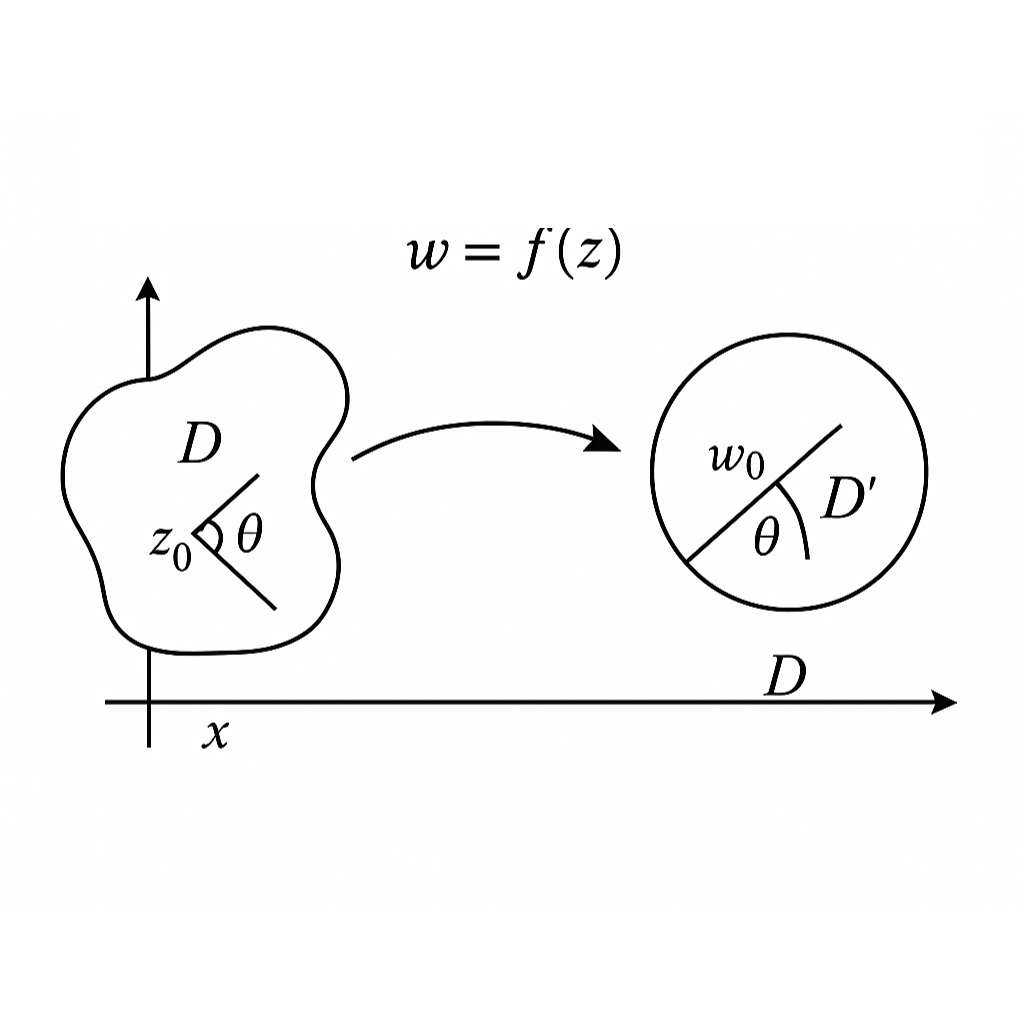
\includegraphics[width=0.9\textwidth]{Images/SC Intro.png}
\caption{Schwarz-Christoffel transformation overview}
\end{figure}

\begin{center}\rule{0.5\linewidth}{0.5pt}\end{center}

\newpage
\tableofcontents

\newpage
\section{Introduction to Conformal
Mapping}\label{introduction-to-conformal-mapping-1}

The study of conformal mapping is a cornerstone of complex analysis,
providing a powerful mathematical framework for solving boundary value
problems in two dimensions. A conformal map is a function that preserves
the angles between intersecting curves, both in magnitude and sense
(orientation). This property is invaluable in transforming complex
geometries into simpler, standard domains where solutions to physical
problems, such as those governed by Laplace's equation, are readily
available. The ability to transform a complex physical domain into a
simple computational domain, solve the problem there, and then map the
solution back to the physical domain is the central utility of conformal
mapping. This technique is not just a mathematical curiosity but a
practical tool that has shaped the fields of fluid dynamics,
electrostatics, and computational geometry. The preservation of the
governing equations (like Laplace's equation) under conformal
transformation is the key mathematical property that makes this approach
so effective. This report will focus on the most explicit and
constructive tool in this domain: \textbf{the Schwarz-Christoffel
Transformation}.

\begin{figure}[h]
\centering
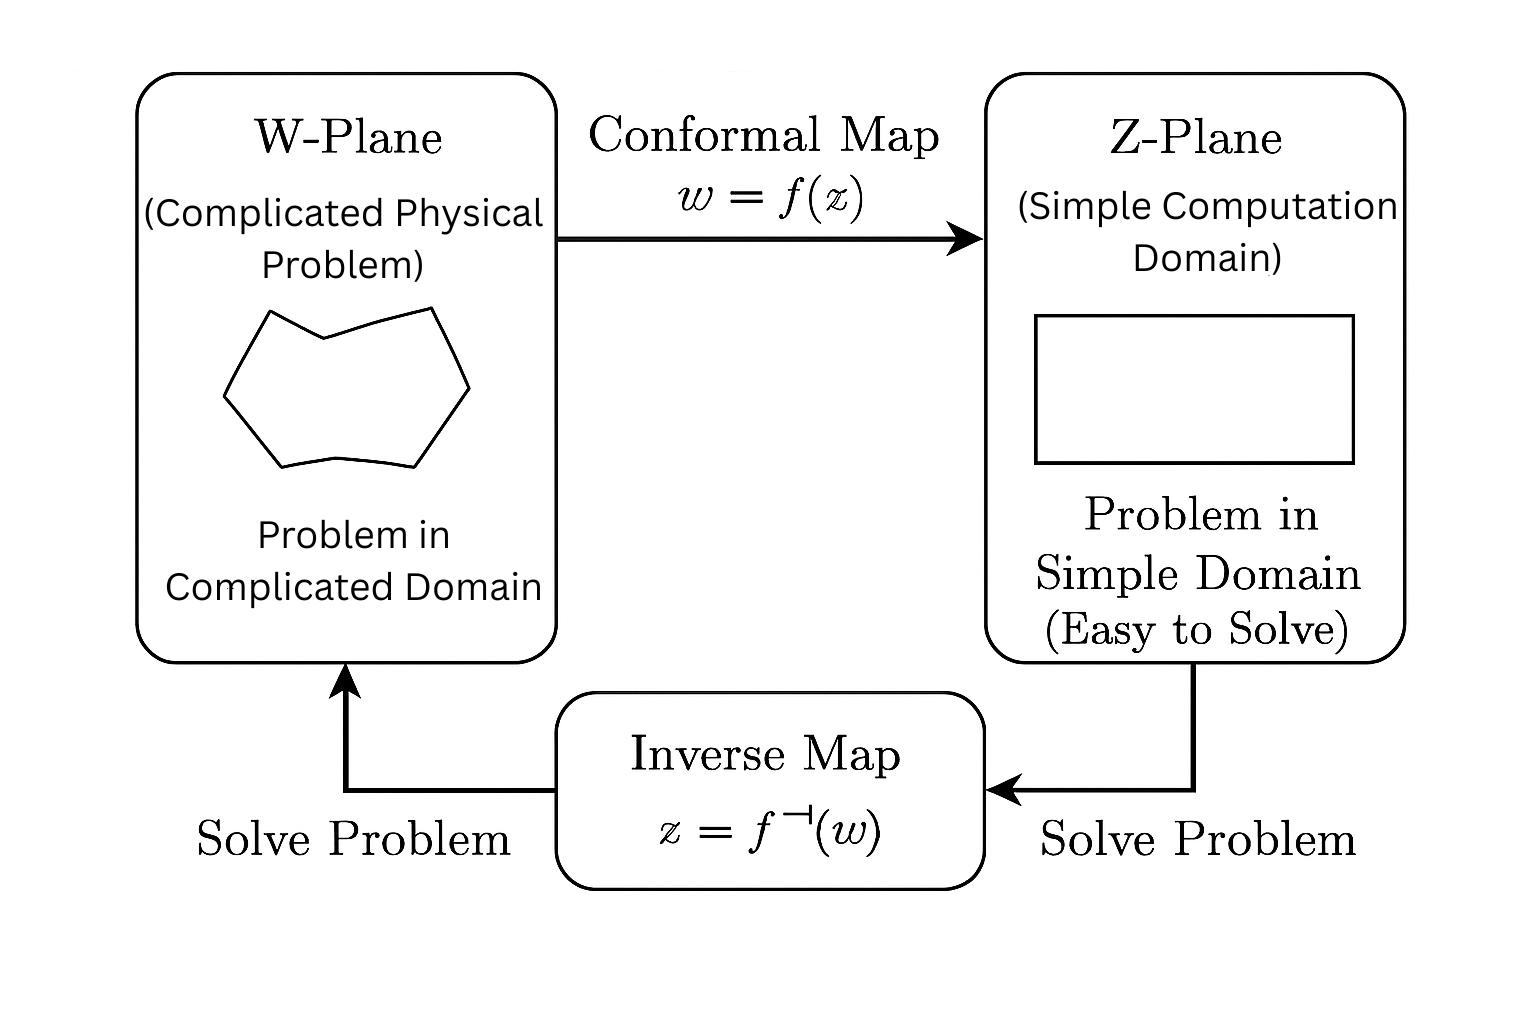
\includegraphics[width=1\textwidth]{Images/conformal_mapping_utility_diagram.png}
\caption{Transformation illustration}
\end{figure}

The ability of conformal maps to preserve local shape, while allowing for global
distortion, is what makes them so powerful. This preservation of angles
is mathematically equivalent to the mapping function being analytic, a
condition that forms the bedrock of complex analysis and its
applications to physical problems. The transformation effectively allows
engineers and physicists to solve complex boundary value problems in a
simplified domain and then map the solution back to the original,
intricate geometry.

\subsection{Historical Context and
Foundations}\label{historical-context-and-foundations}

The concept of angle-preserving transformations has roots dating back to
ancient cartography, notably with Claudius Ptolemy's stereographic
projection and Gerhard Kremer's Mercator projection in 1569 .
However, the rigorous mathematical foundation was established much
later. Carl Friedrich Gauss first solved the general problem of
determining all conformal mappings for a small neighborhood of a point
in 1822 .

The major breakthrough came with \textbf{Bernhard Riemann} in 1851, who
formulated the \textbf{Riemann Mapping Theorem}. While Riemann's initial
proof relied on the assumption that the Dirichlet problem had a
solution, the theorem was later rigorously established by
\textbf{Hermann Schwarz} in 1890 and \textbf{David Hilbert} in 1901
. The historical development of computational methods, including
the work of Lichtenstein (1917) and Theodorsen (1931), highlights the
continuous effort to find practical ways to compute these complex
transformations .

The first numerical research into developing a method for
mapping a region bounded by finitely many Jordan curves was done by
Burnside in 1891 . A minimizing principle was established by
\textbf{Bieberbach} in 1914, namely, that among all suitably normed
conformal maps of a given simply connected region the one with the least
area is the conformal map onto a circle . The development of
integral equation methods by \textbf{Lichtenstein} in 1917, who reduced
the problem to the solution of an integral equation, marked a
significant step forward . Other attempts in this direction were
made by Krylov and Bogolyubov in 1929. A significant contribution was
made by \textbf{Nyström} in 1930, who gave a method for an approximate
solution of integral equations useful in conformal mapping . The
important result known as \textbf{Theodorsen's integral equation} was
developed in 1931 for conformally mapping nearly circular regions onto a
circle, which further solidified the field's practical application
. This historical trajectory highlights the continuous shift from
purely theoretical existence proofs to practical, computational methods
for constructing conformal maps, often involving the solution of complex
integral equations.

\subsection{Analytic Functions and
Conformality}\label{analytic-functions-and-conformality}

The mathematical condition for a transformation \(w = f(z)\) to be
conformal is intrinsically linked to the properties of \textbf{analytic
functions}. A function \(f(z)\) is analytic (or holomorphic) in a region
\(D\) if its derivative \(f'(z)\) exists at every point in \(D\).

The necessary condition for analyticity is the
\textbf{Cauchy-Riemann Equations}:

\begin{formulabox}
\[\frac{\partial u}{\partial x} = \frac{\partial v}{\partial y} \quad \text{and} \quad \frac{\partial u}{\partial y} = -\frac{\partial v}{\partial x}\]
where \(f(z) = u(x, y) + iv(x, y)\).
\end{formulabox}

The connection to conformal mapping is direct:

\begin{definitionbox}
\begin{itemize}
\item \textbf{Sufficient Condition:} If \(f(z)\) is analytic in domain \(D\) and its derivative
\(f'(z) \neq 0\) for all \(z \in D\), then \(f(z)\) is a conformal
mapping in \(D\).
\item \textbf{Local Univalence:} The condition
\(f'(z) \neq 0\) ensures that the mapping is locally one-to-one
(injective), meaning small neighborhoods map to small neighborhoods
without overlap.
\item \textbf{Harmonic Functions:} The real and imaginary
parts of an analytic function, \(u\) and \(v\), are \textbf{harmonic
functions} (i.e., they satisfy Laplace's equation, \(\nabla^2 u = 0\)
and \(\nabla^2 v = 0\)). This property is crucial because it allows
boundary value problems defined by Laplace's equation to be solved in
the simpler transformed domain.
\end{itemize}
\end{definitionbox}

\subsubsection{Properties of Conformal
Mapping}\label{properties-of-conformal-mapping}

A key property of conformal maps is the preservation of orthogonality,
which is a direct consequence of the Cauchy-Riemann equations. The level
curves of \(u(x, y) = \text{constant}\) and
\(v(x, y) = \text{constant}\) are orthogonal at every point where
\(f'(z) \neq 0\).

\textbf{Local Scale Factor:} While angles are preserved, distances are
not. However, the ratio of infinitesimal distances is preserved, which
is defined by the \textbf{local scale factor} or \textbf{magnification
factor}, \(\lambda\): \[
\lambda = |f'(z)| = \left| \frac{dw}{dz} \right|
\] This factor is independent of the direction of the curve at \(z\). If
\(ds_w\) is an infinitesimal length in the \(w\)-plane and \(ds_z\) is
the corresponding length in the \(z\)-plane, then
\(ds_w = \lambda ds_z\). This means that a small circle centered at
\(z\) is mapped to a small circle centered at \(w=f(z)\), but with a
radius scaled by \(\lambda\).

\textbf{Preservation of Orientation:} Conformal maps also preserve the
orientation (sense) of the angle. A mapping that preserves the magnitude
of angles but reverses the orientation is called an \textbf{isogonal}
mapping. For an analytic function \(f(z)\), the derivative \(f'(z)\) is
a complex number whose argument, \(\arg(f'(z))\), represents the angle
of rotation of the tangent vector at \(z\).


\begin{figure}
\centering
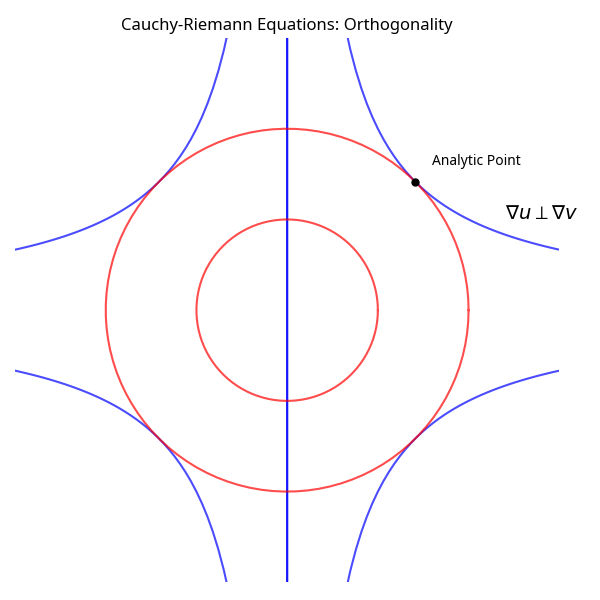
\includegraphics[width=0.7\textwidth]{Images/cauchy_riemann.png}
\caption{Cauchy-Riemann Orthogonality}
\end{figure}

\begin{center}\rule{0.5\linewidth}{0.5pt}\end{center}

\newpage
\section{Foundational Theorems of Conformal
Mapping}\label{foundational-theorems-of-conformal-mapping-2}

\subsection{The Riemann Mapping
Theorem}\label{the-riemann-mapping-theorem}

The \textbf{Riemann Mapping Theorem} is the foundational result that
guarantees the existence of a conformal map for a vast class of domains.

\begin{theorembox}
\textbf{Theorem (Riemann Mapping Theorem):} Let \(D \subset \mathbb{C}\) be a simply connected
region, and \(D \neq \mathbb{C}\). Then there exists a conformal mapping
\(f : D \to U\) that maps \(D\) onto the open unit disk
\(U = \{w \in \mathbb{C} : |w| < 1\}\).
\end{theorembox}

The theorem has profound significance:

\begin{importantbox}
\begin{itemize}
\item \textbf{Existence:} It
guarantees that a conformal mapping from any simply connected domain
(excluding the entire complex plane) to the unit disk always exists.

\item \textbf{Uniqueness:} The mapping is unique up to normalization (e.g.,
fixing the image of a point and the argument of the derivative at that
point).

\item \textbf{Significance:} This theorem enables the reduction of
complex boundary value problems defined on arbitrary simply connected
domains to standard problems on the unit disk, where solutions are
well-known.
\end{itemize}
\end{importantbox}

The theorem essentially states that all simply connected domains, no
matter how complex their boundary, are conformally equivalent to the
simplest possible domain, the unit disk. The uniqueness of the mapping
is a critical aspect, ensuring that once the normalization conditions
are fixed (e.g., fixing the image of a point and the argument of the
derivative at that point), the conformal map is uniquely determined.
This property is vital for applications, as it guarantees a consistent
and predictable transformation for solving boundary value problems. The
rigorous proof of the theorem, completed by Schwarz and Hilbert,
confirmed the foundational role of this concept in complex analysis.

\begin{figure}[h]
\centering
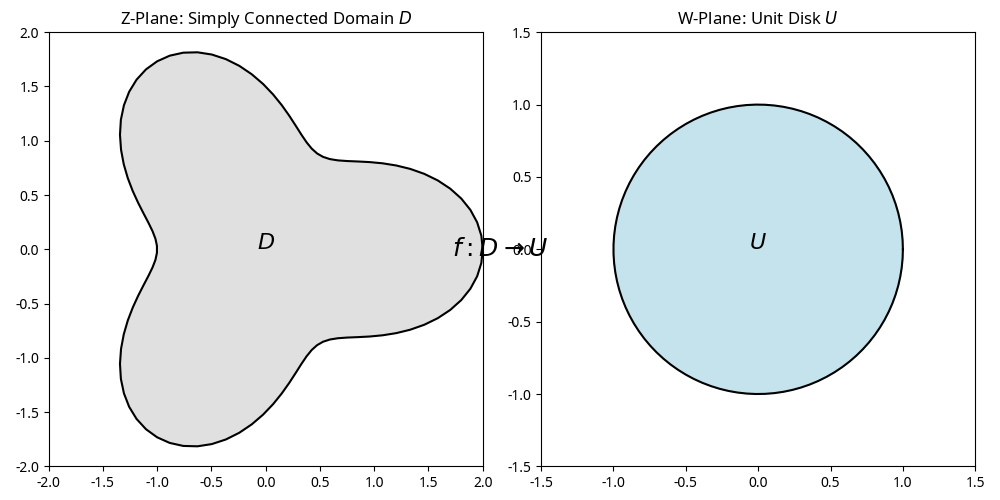
\includegraphics[width=0.75\textwidth]{Images/riemann_mapping.png}
\caption{Riemann Mapping Theorem Concept}
\end{figure}

\subsection{The Bilinear (Möbius)
Transformation}\label{the-bilinear-muxf6bius-transformation}

A simple, yet powerful, class of conformal maps is the \textbf{Bilinear
(Möbius) Transformation}, defined by: \[
w = \frac{az+b}{cz+d}, \quad \text{where } ad - bc \neq 0
\]

This transformation is conformal everywhere except at the pole
\(z = -d/c\). Its key properties are:

\begin{importantbox}
\begin{itemize}
\item \textbf{Circle/Line Preservation:} It maps circles and straight lines in the \(z\)-plane to
circles or straight lines in the \(w\)-plane. Straight lines are
considered circles with infinite radius.

\item \textbf{Composition:} Any
bilinear transformation can be decomposed into a sequence of simpler
transformations: translation, rotation/magnification, and inversion.

\item \textbf{Normalization:} The condition \(ad - bc \neq 0\) ensures the
transformation is non-degenerate and invertible.
\end{itemize}
\end{importantbox}

A common application is mapping the upper half-plane (UHP) to the unit
disk, as illustrated below. The transformation
\(w = \frac{z-z_0}{z-\bar{z}_0}\) maps the UHP to the unit disk, where
\(z_0\) is a point in the UHP. The decomposition of the Bilinear
Transformation is particularly insightful: it can be viewed as a
sequence of elementary transformations:

\begin{enumerate}
\item \textbf{Translation:} \(z_1 = z + d/c\)
\item \textbf{Inversion:} \(z_2 = 1/z_1\)
\item \textbf{Rotation and Magnification:} \(w = \frac{ad-bc}{c} z_2 + \frac{a}{c}\)
\end{enumerate}

This decomposition
demonstrates the fundamental nature of the Bilinear Transformation,
showing how complex mappings can be built from simple geometric
operations. Its property of mapping circles and lines to circles and
lines makes it an indispensable tool for simplifying domains in the
initial stages of a conformal mapping problem.

Furthermore, the Bilinear Transformation is involutory when
\(w = \frac{az+b}{cz+d}\) and \(z = \frac{dw-b}{-cw+a}\), which occurs
when \(a = -d\). This property is important in certain geometric
applications where the transformation is its own inverse.

The Bilinear Transformation is often used as a preliminary step in more
complex mappings, allowing for the standardization of one part of the
domain before applying a more specialized transformation like the
Schwarz-Christoffel formula.

\paragraph{Decomposition of the Bilinear
Transformation}\label{decomposition-of-the-bilinear-transformation}

The Bilinear Transformation, a fundamental conformal map, can be
understood as a sequence of simpler geometric operations: translation,
inversion, and rotation/magnification. This decomposition is crucial for
understanding how complex maps are built from elementary
transformations.

\begin{figure}[h]
\centering
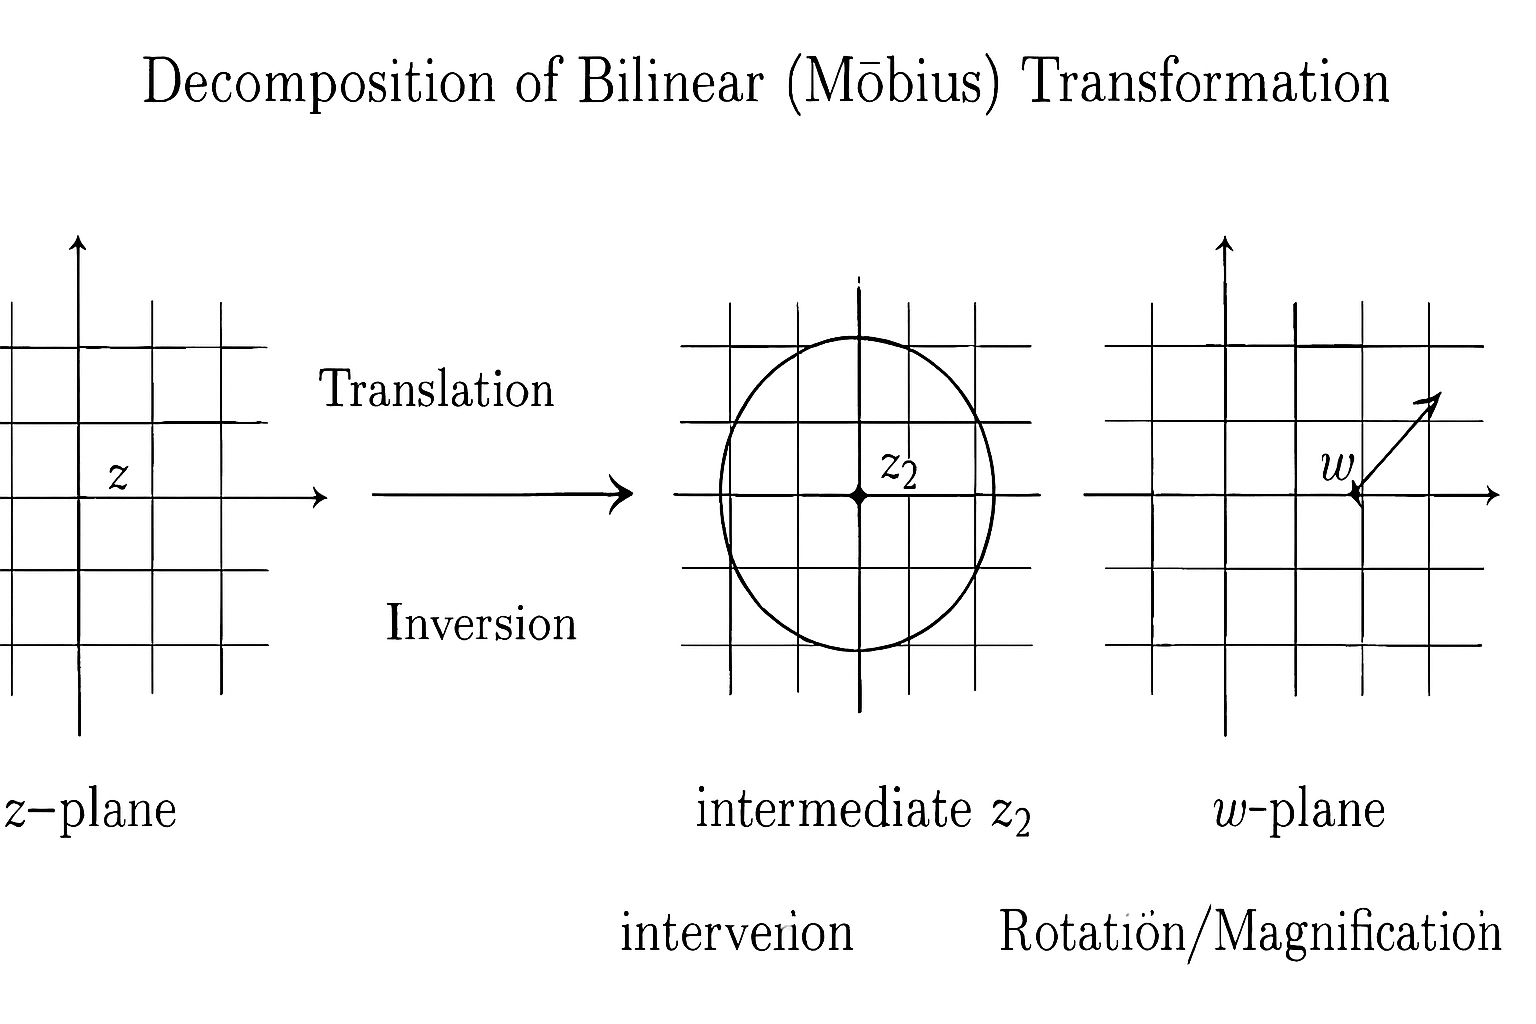
\includegraphics[width=0.8\textwidth]{Images/bilinear_decomposition.png}
\caption{Bilinear Transformation Decomposition}
\end{figure}

\begin{center}\rule{0.5\linewidth}{0.5pt}\end{center}

\newpage
\section{The Schwarz-Christoffel
Transformation}\label{the-schwarz-christoffel-transformation-1}

While the Riemann Mapping Theorem guarantees the existence of a
conformal map, it does not provide an explicit formula for constructing
it for an arbitrary domain. The \textbf{Schwarz-Christoffel (SC)
Transformation} fills this gap for a specific, yet highly important,
class of domains: simple polygons.

\subsection{Purpose and General
Formula}\label{purpose-and-general-formula}

The SC transformation maps the upper half-plane (UHP),
\(\text{Im}(z) > 0\), conformally onto the interior of any simple
polygon with a finite number of vertices.

The differential form of the SC transformation is given by:

\begin{formulabox}
\[\frac{dw}{dz} = A \prod_{k=1}^{n} (z - x_k)^{-\alpha_k}\]
\end{formulabox}

The mapping function \(w = f(z)\) is obtained by integrating this
expression:

\begin{formulabox}
\[w = A \int \prod_{k=1}^{n} (z - x_k)^{-\alpha_k} dz + B\]
\end{formulabox}

Where:
\begin{itemize}
\item \(w\) is the complex coordinate in the polygon plane.
\item \(z\) is the complex coordinate in the upper half-plane.
\item \(x_k\) are
\(n\) distinct points on the real axis of the \(z\)-plane
(\(x_1 < x_2 < \cdots < x_n\)) that map to the vertices \(w_k\) of the
polygon in the \(w\)-plane.
\item \(\alpha_k \pi\) is the \textbf{exterior
angle} at the vertex \(w_k\).
\item \(A\) and \(B\) are complex constants
determined by normalization conditions.
\end{itemize}

The interior angle \(\theta_k\) of the polygon at vertex \(w_k\) is
related to the exterior angle \(\alpha_k \pi\) by:

\begin{importantbox}
\[\theta_k = (1 - \alpha_k)\pi \quad \text{or} \quad \alpha_k = 1 - \frac{\theta_k}{\pi}\]

For a closed polygon with \(n\) vertices, the sum of the exterior
angles is \(2\pi\), which implies: \(\sum_{k=1}^{n} \alpha_k = 2\).
\end{importantbox}

The general concept of the mapping is illustrated below, showing the
pre-images \(x_k\) on the real axis mapping to the vertices \(w_k\) of
the polygon.

\subsection{Derivation Concept: The Argument
Principle}\label{derivation-concept-the-argument-principle}

\textbf{The Argument Principle:} The core idea behind the SC formula is to control the change in the
argument (angle) of the derivative \(\frac{dw}{dz}\) as the point \(z\)
moves along the real axis of the UHP.

\textbf{Boundary Mapping:} The real axis in the \(z\)-plane
maps to the boundary of the polygon in the \(w\)-plane. As \(z\)
traverses the real axis from left to right, the image point \(w\) traces
the polygon boundary.

\textbf{Vertex Control:} At each vertex \(w_k\), the path must turn by the
exterior angle \(\alpha_k \pi\).

\begin{figure}[h]
\centering
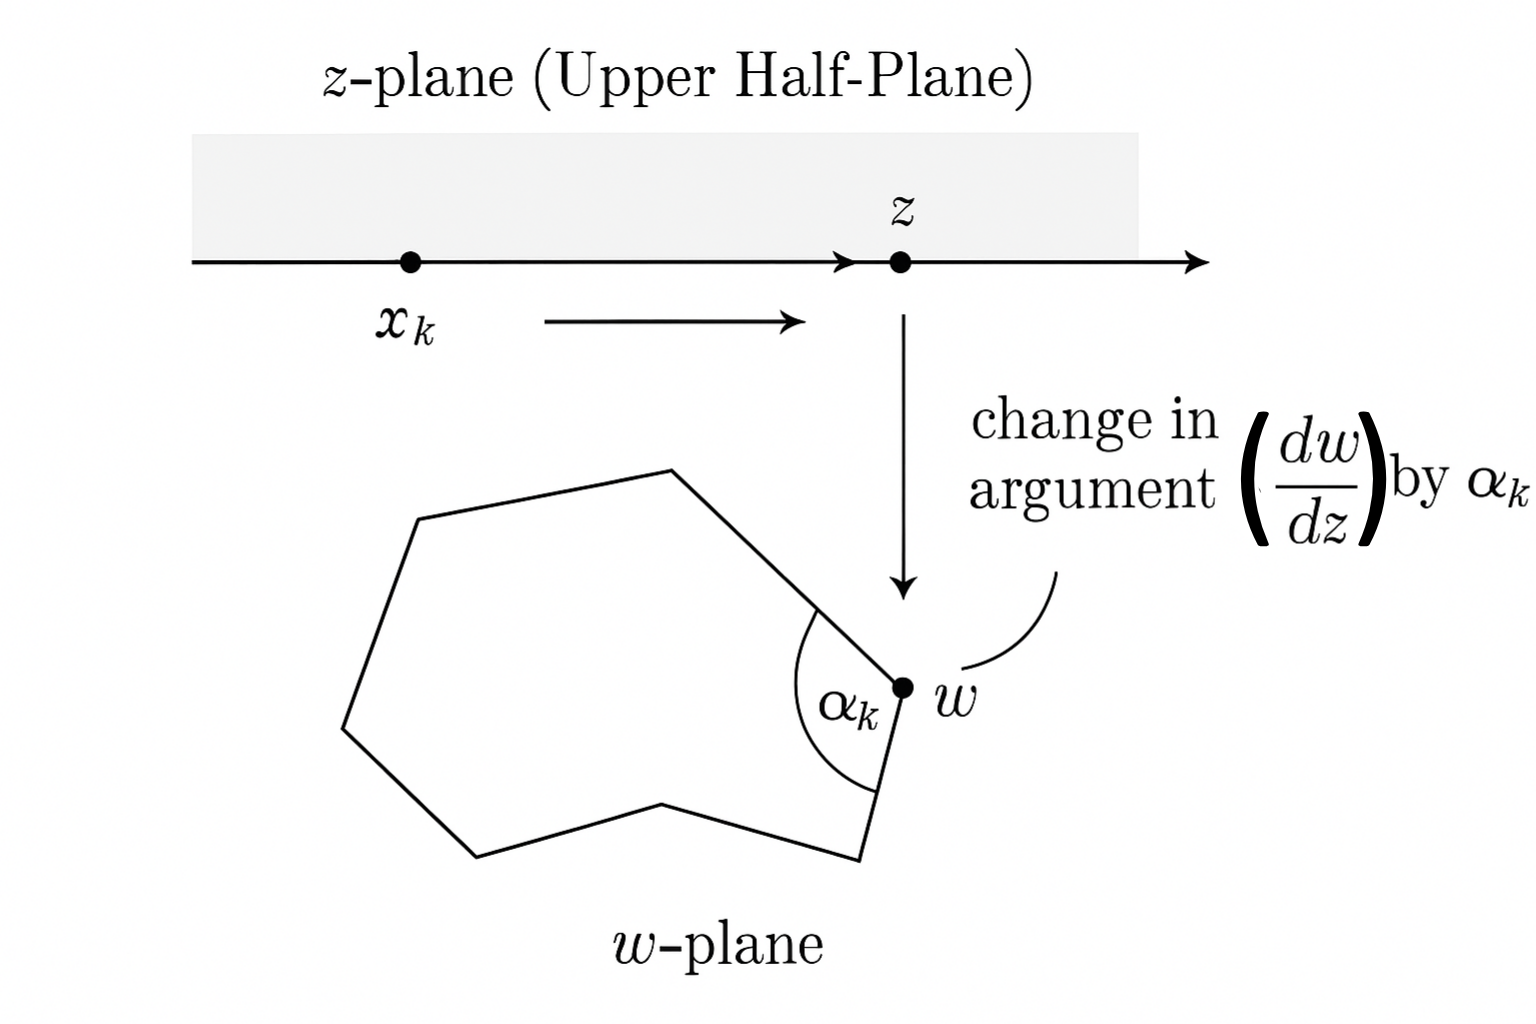
\includegraphics[width=0.75\textwidth]{Images/sc_derivation_concept.png}
\caption{SC Derivation Concept}
\end{figure}

\begin{formulabox}
\textbf{Schwarz-Christoffel Formula:}
\[
\frac{dw}{dz} = A \prod_{k=1}^{n} (z - x_k)^{-\alpha_k}
\]
where \(A\) is a complex constant, \(x_k\) are the pre-images of the polygon vertices on the real axis, and \(\alpha_k\) are the exterior angles.
\end{formulabox}

\begin{importantbox}
\textbf{Why \((z - x_k)^{-\alpha_k}\)?}

As \(z\) crosses \(x_k\) on the real axis (moving from \(x_k - \epsilon\) to \(x_k + \epsilon\) via the upper half-plane), the argument of \((z - x_k)\) changes by \(-\pi\).

Therefore, the argument of \((z - x_k)^{-\alpha_k}\) changes by:
\[
\Delta \arg((z - x_k)^{-\alpha_k}) = -\alpha_k \times (-\pi) = \alpha_k \pi
\]

This is exactly the exterior angle turn required at vertex \(w_k\).
\end{importantbox}

\begin{theorembox}
\textbf{Exterior Angle Relationship:}
\begin{itemize}
\item Interior angle at vertex \(k\): \(\theta_k = (1 - \alpha_k)\pi\)
\item Exterior angle at vertex \(k\): \(\alpha_k \pi\)
\item Constraint: \(\sum_{k=1}^{n} \alpha_k = 2\) (ensures polygon closes)
\end{itemize}
\end{theorembox}



\subsubsection{Step-by-Step Derivation
Concept}\label{step-by-step-derivation-concept}

\begin{enumerate}
\def\labelenumi{\arabic{enumi}.}
\item
  \textbf{Start with the derivative:} We seek a function \(w = f(z)\) that maps the upper half-plane conformally to a polygon. The derivative \(\frac{dw}{dz}\) encodes how angles and shapes are transformed.

\item
  \textbf{Control the argument:} As \(z\) moves along the real axis, the argument of \(\frac{dw}{dz}\) must change by the exterior angle \(\alpha_k \pi\) at each vertex pre-image \(x_k\).

\item
  \textbf{Construct the product form:} Each factor \((z - x_k)^{-\alpha_k}\) contributes the required argument change \(\alpha_k \pi\) as \(z\) crosses \(x_k\). The product of all such factors ensures simultaneous control at all vertices.

\item
  \textbf{Integrate to find \(w\):} The mapping function is obtained by integrating:
  \[
  w = A \int \prod_{k=1}^{n} (z - x_k)^{-\alpha_k} \, dz + B
  \]
  where \(A\) and \(B\) are complex constants controlling scale, rotation, and translation.
\end{enumerate}

\subsubsection{Construction Steps}\label{construction-steps}

\begin{enumerate}
\def\labelenumi{\arabic{enumi}.}
\item
  \textbf{Identify vertices:} Identify vertices \(x_1, x_2, \ldots, x_n\) on the real axis that map to polygon vertices \(w_1, w_2, \ldots, w_n\).

\item
  \textbf{Determine exterior angles:} Determine exterior angles \(\alpha_k \pi\) from the interior angles \(\theta_k\) of the polygon.

\item
  \textbf{Construct the product:} Construct the product \(\prod_{k=1}^{n} (z - x_k)^{-\alpha_k}\) to ensure each factor contributes the correct argument change.

\item
  \textbf{Integrate to obtain \(w\):} Integrate to obtain
  \[
  w = A \int \prod_{k=1}^{n} (z - x_k)^{-\alpha_k} \, dz + B
  \]
  where \(A\) and \(B\) are determined by normalization conditions.
\end{enumerate}

\begin{figure}[h]
\centering
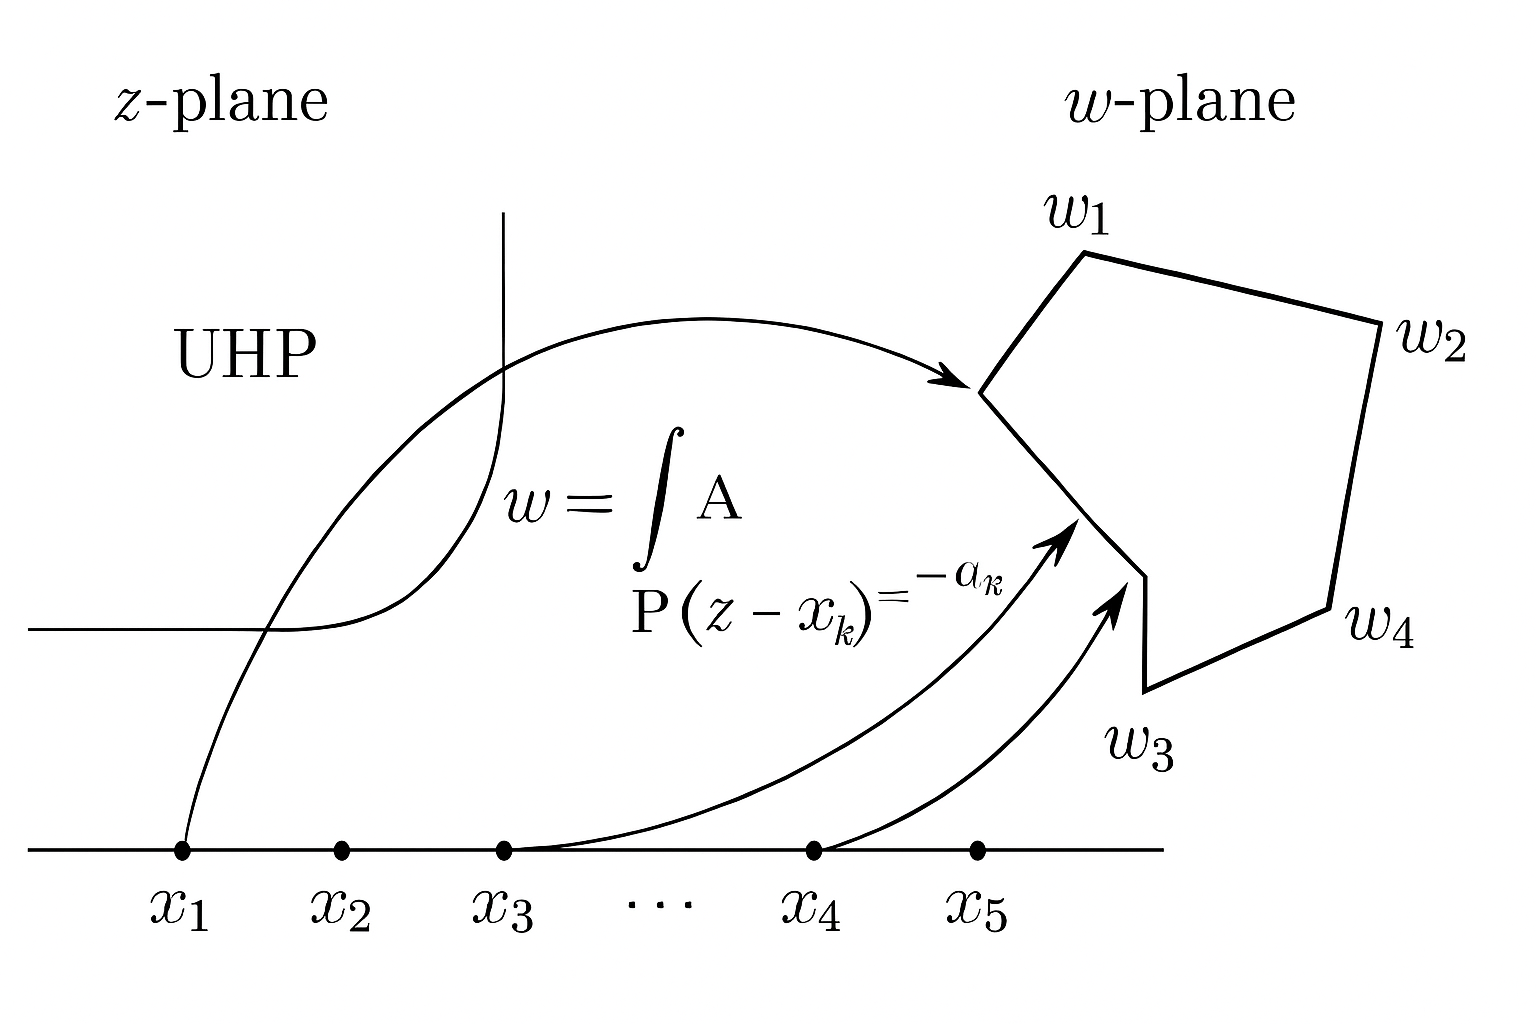
\includegraphics[width=0.75\textwidth]{Images/sc_formula_diagram.png}
\caption{SC Formula Diagram}
\end{figure}

\subsection{Parameters of the
Transformation}\label{parameters-of-the-transformation}

The SC formula involves \(n\) pre-images \(x_k\) on the real axis, \(n\)
exterior angles \(\alpha_k\), and two complex constants \(A\) and \(B\).

\textbf{The Location of Pre-images (\(x_k\)):} The location of the \(n\)
points \(x_k\) on the real axis determines the relative lengths of the
sides of the polygon. For a polygon with \(n\) vertices, only \(n - 3\)
of the pre-image points can be chosen arbitrarily. The remaining three
points are fixed by the choice of the constants \(A\) and \(B\), which
control the scale, rotation, and translation of the resulting polygon.
This freedom of choice is a consequence of the fact that a bilinear
transformation can map any three points on the real axis to any other
three points on the real axis, and the composition of a conformal map
with a bilinear map is still a conformal map.

\textbf{The Constants \(A\) and \(B\):}

\begin{itemize}
\item \textbf{Constant \(A\) (Scale
and Rotation):} The magnitude \(|A|\) determines the size (scale) of the
polygon, and the argument \(\arg(A)\) determines its orientation
(rotation) in the \(w\)-plane.

\item \textbf{Constant \(B\) (Translation):}
The constant \(B\) determines the position (translation) of the polygon
in the \(w\)-plane.
\end{itemize}

In practical applications, the values of \(x_k\), \(A\), and \(B\) are
chosen to match the desired dimensions and location of the target
polygon. This often involves solving a system of non-linear equations,
which can be computationally intensive for complex polygons.

\paragraph{The Parameter Problem in Schwarz-Christoffel
Mapping}\label{the-parameter-problem-in-schwarz-christoffel-mapping}

The parameter problem is the challenge of determining the pre-image
points \(x_k\) on the real axis that correspond to the desired side
lengths of the target polygon. This is a non-linear problem central to
the practical application of the SC formula.

\begin{center}\rule{0.5\linewidth}{0.5pt}\end{center}

\newpage
\section{Examples of SC
Mapping}\label{examples-of-sc-mapping-1}

The power of the Schwarz-Christoffel transformation lies in its ability
to provide an explicit, albeit sometimes complex, integral form for the
mapping function of various polygonal regions.

\subsection{Mapping to a Rectangle and Elliptic
Integrals}\label{mapping-to-a-rectangle-and-elliptic-integrals}

Mapping the UHP onto a rectangle is a classic example that demonstrates
the complexity of the SC integral. A rectangle has four vertices, each
with an interior angle of \(\theta_k = \pi/2\).

\begin{formulabox}
The exterior angle is \(\alpha_k \pi\), where \[
\alpha_k = 1 - \frac{\pi/2}{\pi} = 1 - \frac{1}{2} = \frac{1}{2}
\] Since there are four vertices, \(n=4\), and all \(\alpha_k = 1/2\).
The differential equation becomes: \[
\frac{dw}{dz} = A (z - x_1)^{-1/2} (z - x_2)^{-1/2} (z - x_3)^{-1/2} (z - x_4)^{-1/2} = \frac{A}{\sqrt{(z-x_1)(z-x_2)(z-x_3)(z-x_4)}}
\] The mapping function is: \[
w = A \int \frac{dz}{\sqrt{(z-x_1)(z-x_2)(z-x_3)(z-x_4)}} + B
\]
\end{formulabox}

The integral of this form is known as an \textbf{elliptic integral}.
This demonstrates that even for a simple polygon like a rectangle, the
mapping function cannot be expressed in terms of elementary functions,
highlighting the need for numerical methods in practical SC
applications. The ratio of the sides of the rectangle is determined by
the ratio of two elliptic integrals, which is a key result in the theory
of elliptic functions.

\begin{figure}[h]
\centering
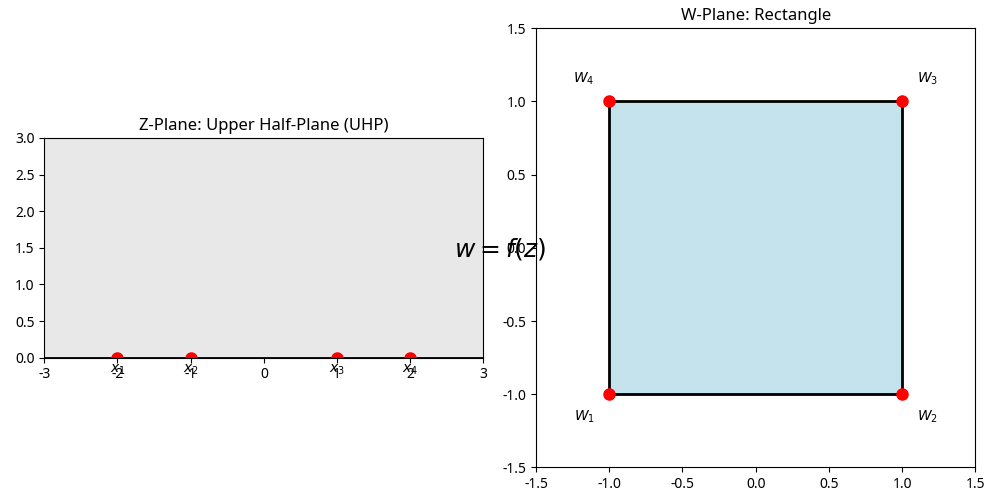
\includegraphics[width=0.75\textwidth]{Images/sc_rectangle.png}
\caption{Rectangular Mapping Concept}
\end{figure}

\subsection{Mapping to a Semi-Infinite
Strip}\label{mapping-to-a-semi-infinite-strip}

A semi-infinite strip is a polygon with three vertices, two at a finite
distance and one at infinity. Consider a strip defined by
\(0 < \text{Im}(w) < h\) and \(\text{Re}(w) > 0\). The vertices are
\(w_1 = 0\), \(w_2 = ih\), and \(w_3 = \infty\).

The interior angles are \(\theta_1 = \pi/2\) and \(\theta_2 = \pi/2\).
The exterior angles are \(\alpha_1 \pi\) with \(\alpha_1 = 1/2\), and 
\(\alpha_2 \pi\) with \(\alpha_2 = 1/2\). Since one vertex is at infinity, we only need two finite pre-images,
\(x_1\) and \(x_2\). Let \(x_1 = -1\) and \(x_2 = 1\).


\begin{formulabox}
The differential equation is: \[
\frac{dw}{dz} = A (z - (-1))^{-1/2} (z - 1)^{-1/2} = \frac{A}{\sqrt{z^2 - 1}}
\] The mapping function is: \[
w = A \int \frac{dz}{\sqrt{z^2 - 1}} + B = A \cosh^{-1}(z) + B
\] By choosing \(A = h/\pi\) and \(B = ih/2\), the mapping becomes:
\[w = \frac{h}{\pi} \cosh^{-1}(z) + \frac{ih}{2}\]
\end{formulabox}

This maps the UHP to the semi-infinite strip. This is a case where the integral can be
solved in terms of elementary functions, providing a closed-form
solution.

\begin{figure}[h]
\centering
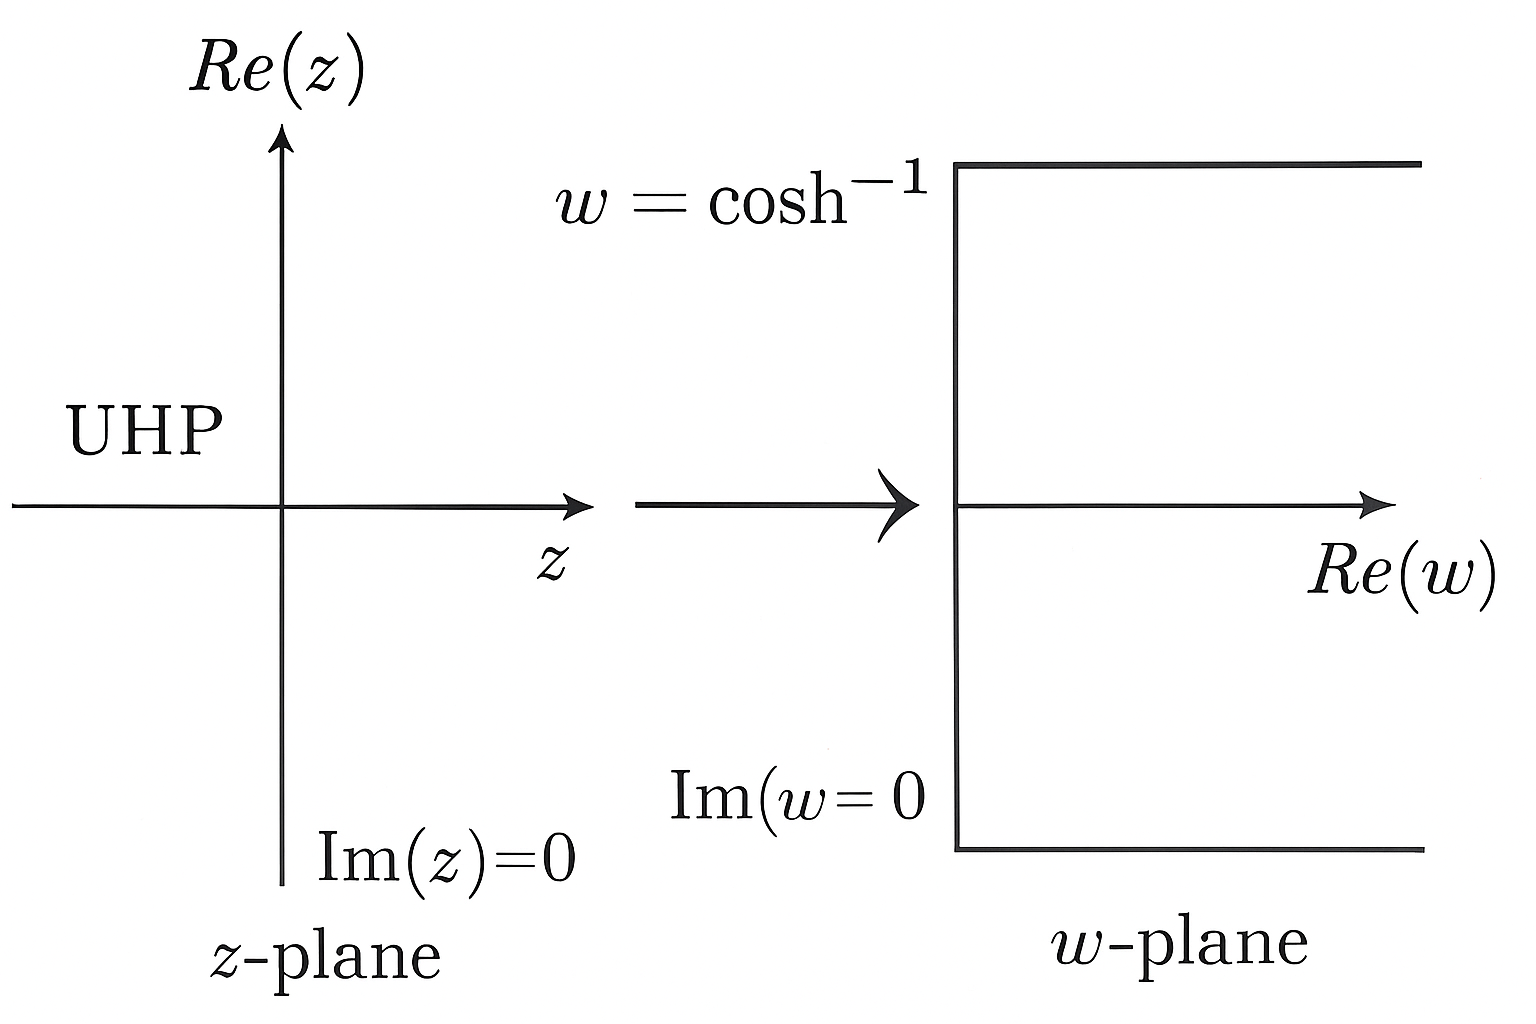
\includegraphics[width=0.75\textwidth]{Images/semi_infinite_strip_mapping.png}
\caption{Semi-Infinite Strip Mapping Concept}
\end{figure}

\subsection{Mapping to a Triangular
Region}\label{mapping-to-a-triangular-region}

A triangle is the simplest closed polygon, with three vertices
\(w_1, w_2, w_3\) and interior angles \(\theta_1, \theta_2, \theta_3\).
The exterior angles are \(\alpha_k = 1 - \theta_k/\pi\). Since
\(\sum \theta_k = \pi\), the sum of the exterior angles is
\(\sum \alpha_k = 3 - \sum \theta_k/\pi = 3 - 1 = 2\), which satisfies
the closure condition.

\begin{formulabox}
The SC formula for a triangle with finite pre-images \(x_1, x_2, x_3\)
is: \[
w = A \int (z - x_1)^{-\alpha_1} (z - x_2)^{-\alpha_2} (z - x_3)^{-\alpha_3} dz + B
\]
\end{formulabox}

This integral is generally an \textbf{hypergeometric function} and
cannot be solved in terms of elementary functions unless the angles are
specific rational multiples of \(\pi\).

\begin{importantbox}
A common simplification is to map one vertex to infinity, say
\(w_3 \to \infty\). This eliminates the factor \((z - x_3)^{-\alpha_3}\)
from the differential equation, leaving only two finite pre-images
\(x_1\) and \(x_2\). The mapping becomes: \[
w = A \int (z - x_1)^{-\alpha_1} (z - x_2)^{-\alpha_2} dz + B
\]
This form is often easier to handle numerically or analytically for
specific angle combinations.
\end{importantbox}

\begin{figure}[h]
\centering
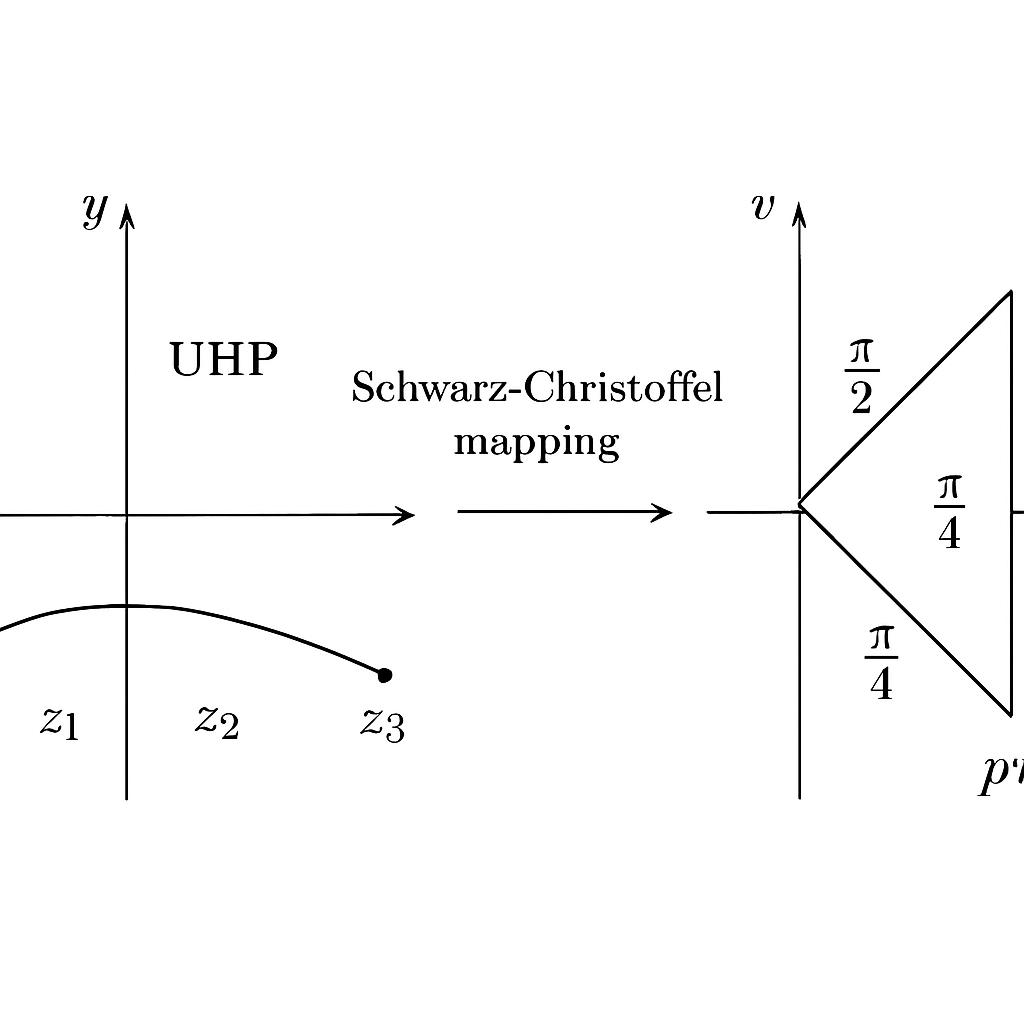
\includegraphics[width=0.75\textwidth]{Images/sc_triangle_mapping.png}
\caption{SC Triangle Mapping Concept}
\end{figure}

\begin{center}\rule{0.5\linewidth}{0.5pt}\end{center}

\newpage
\section{Applications of Conformal Mapping}\label{applications-of-conformal-mapping}

Conformal mapping serves as a powerful mathematical tool for solving complex problems by transforming intricate domains into simpler, more tractable ones. This approach has proven particularly valuable in reducing challenging boundary value problems to standard forms that admit analytical or efficient numerical solutions.

\subsection{Potential Theory and Boundary Value Problems}\label{potential-theory-and-boundary-value-problems}

Conformal mapping provides elegant solutions to Dirichlet and Neumann problems in two dimensions, which are governed by Laplace's equation \(\nabla^2 u = 0\). The technique enables the transformation of complex geometries into canonical domains where boundary value problems can be solved more readily.

\begin{itemize}
\tightlist
\item
  \textbf{Neumann Problem for Laplace's Equation:} Conformal mapping techniques have been successfully applied to solve the Neumann problem for regions exterior to circles, including the determination of Green's functions for such domains. This approach transforms the complex exterior region into a simpler computational domain.

\item
  \textbf{Electrostatic Characterization:} The method of minimizing functionals, closely related to the Plateau problem, provides an electrostatic characterization that serves as an effective approach for determining conformal maps. This connection between variational methods and electrostatics offers both theoretical insight and computational advantages.
\end{itemize}

\begin{figure}[h]
\centering
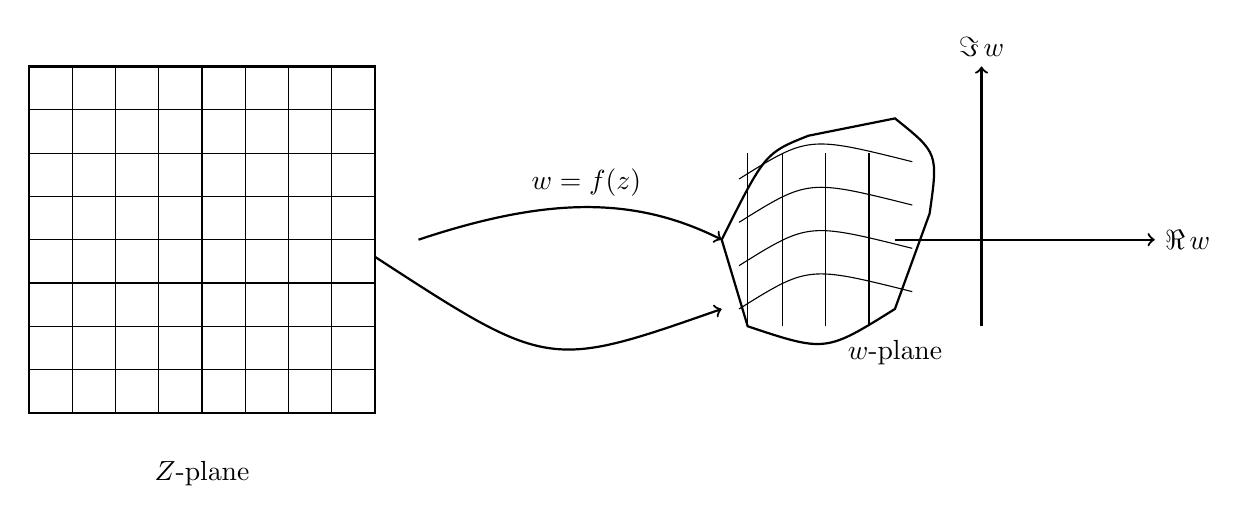
\begin{tikzpicture}[scale=1.1]

%%% --- Z-plane Grid --- %%%
\draw[thick] (0,0) rectangle (4,4);

% vertical grid lines
\foreach \x in {0.5,1,1.5,2,2.5,3,3.5}
  \draw (\x,0) -- (\x,4);

% horizontal grid lines
\foreach \y in {0.5,1,1.5,2,2.5,3,3.5}
  \draw (0,\y) -- (4,\y);

\node at (2,-0.7) {$Z\text{-plane}$};


%%% --- Mapping Arrow --- %%%
\draw[->, thick] (4.5,2) .. controls (6,2.5) and (7,2.5) .. (8,2)
  node[midway, above] {$w = f(z)$};


%%% --- W-plane Axes --- %%%
\draw[->, thick] (10,2) -- (13,2) node[right] {$\Re\,w$};
\draw[->, thick] (11,1) -- (11,4) node[above] {$\Im\,w$};


%%% --- Mapped Irregular Grid (Polygon Domain) --- %%%
\begin{scope}[shift={(8,2)}]
  % boundary polygon
  \draw[thick]
  (0,0) .. controls (0.5,1) .. (1,1.2)
  -- (2,1.4) .. controls (2.5,1) .. (2.4,0.3)
  -- (2,-0.8) .. controls (1.2,-1.3) .. (0.3,-1)
  -- cycle;

  % curved grid lines (rough sketch)
  \foreach \x in {0.3,0.7,1.2,1.7}
    \draw[thin] (\x,-1) .. controls (\x,0.2) .. (\x,1);

  \foreach \y in {-0.8,-0.3,0.2,0.7}
    \draw[thin] (0.2,\y) .. controls (1,\y+0.5) .. (2.2,\y+0.2);

\end{scope}

\node at (10,0.7) {$w\text{-plane}$};


%%% --- Arrow from Z-grid to polygon domain --- %%%
\draw[->, thick] (4,1.8) .. controls (6,0.5) .. (8,1.2);


\end{tikzpicture}
\caption{Conformal mapping from a rectangular grid in the $z$-plane 
to an irregular domain in the $w$-plane.}
\end{figure}

\subsection{Fluid Dynamics and Aerodynamics}\label{fluid-dynamics-and-aerodynamics}

Conformal mapping has extensive applications in fluid mechanics, particularly for analyzing incompressible, irrotational flow problems where complex potential theory applies.

\begin{itemize}
\tightlist
\item
  \textbf{Airfoil Analysis:} The method of small parameters combined with conformal mapping enables the analysis of dynamic problems involving airfoils. This approach allows engineers to study aerodynamic properties and performance characteristics efficiently.

\item
  \textbf{Flow and Heat Transfer in Conduits:} Conformal mapping facilitates the solution of flow and heat transfer problems in rectangular channels and layered geometries. By transforming complex channel cross-sections into simpler domains, the governing equations become more amenable to analytical or numerical solution.

\item
  \textbf{Ideal Fluid Instability:} The technique has been applied to study the Rayleigh-Taylor instability in ideal fluids, where the conformal transformation simplifies the analysis of interfacial dynamics and stability characteristics.

\item
  \textbf{Kirchhoff Flow:} Conformal mapping provides solutions to the classical Kirchhoff flow problem involving flow past polygonal obstacles, enabling the determination of velocity fields and pressure distributions around sharp-cornered bodies.
\end{itemize}

\begin{figure}[h]
\centering
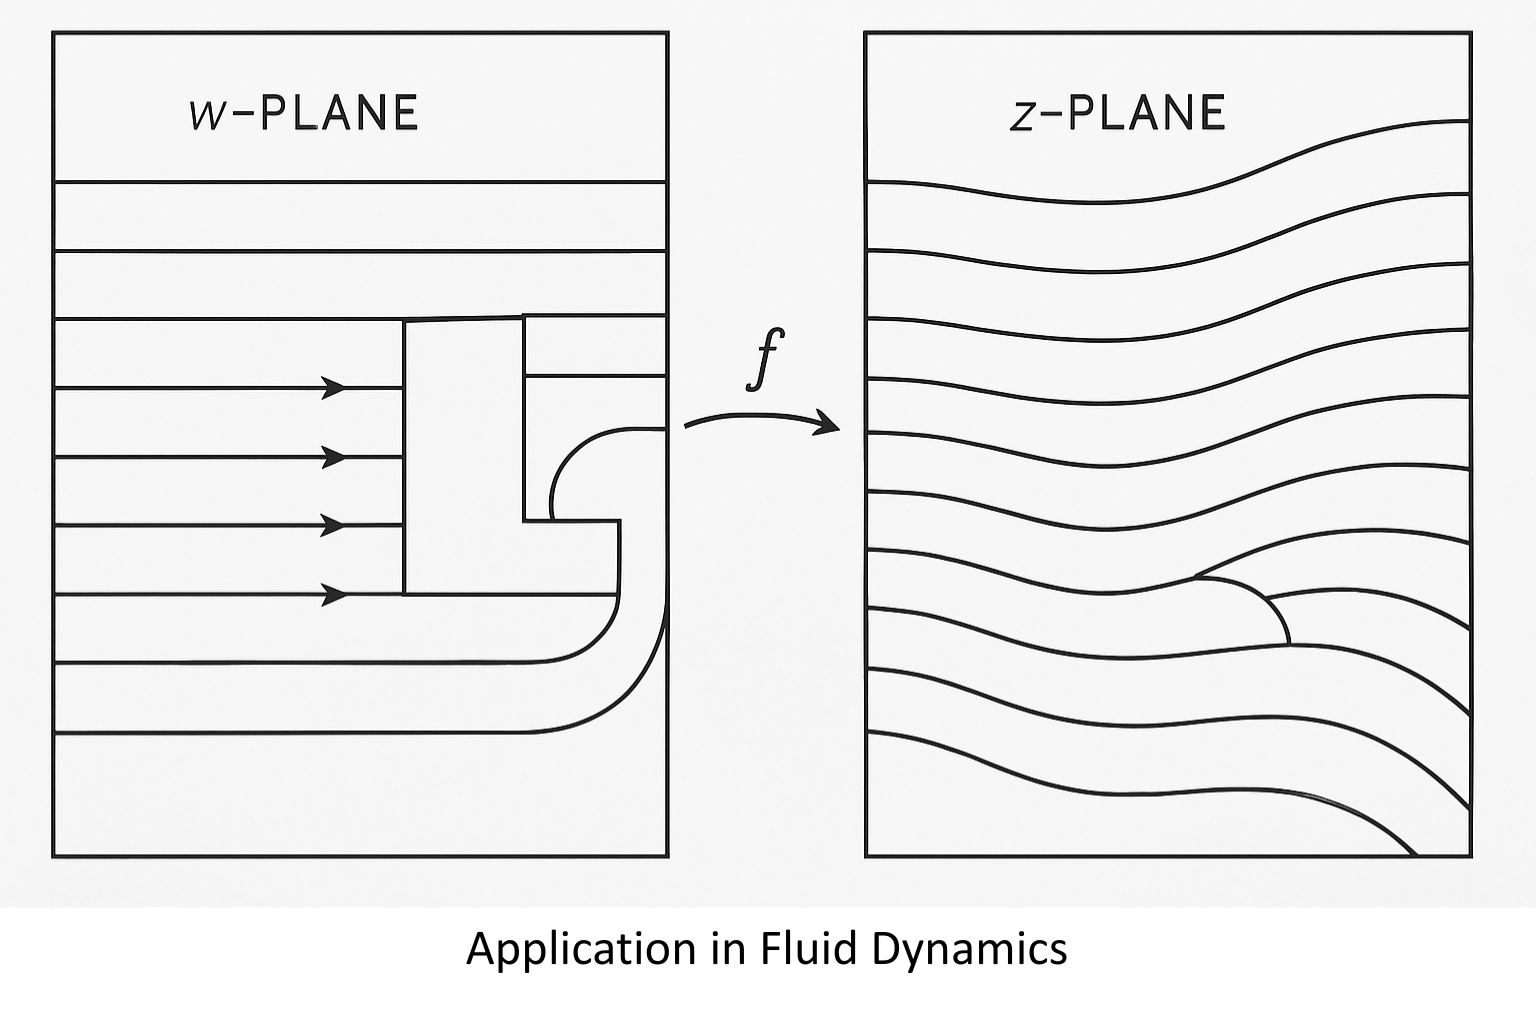
\includegraphics[width=0.8\textwidth]{Images/app-2-fluid-dynamics.png}
\caption{Application of Conformal Mapping in Fluid Dynamics and Aerodynamics}
\end{figure}

\subsection{Engineering and Numerical Methods}\label{engineering-and-numerical-methods}

Modern engineering applications leverage conformal mapping for domain simplification in various computational and analytical contexts.

\begin{itemize}
\tightlist
\item
  \textbf{Thermoelastic Problems:} Conformal mapping assists in solving thermoelastic problems involving uniform heat flow perturbed by isolated holes of complex geometries, such as ovaloid forms. This approach enables the analysis of thermal stress distributions in components with geometric irregularities.

\item
  \textbf{Stress Analysis in Propellant Grains:} The technique is employed to determine stress distributions in solid propellant rocket grains through the solution of integral equations. Mapping complex grain geometries to simpler domains facilitates both analytical and numerical stress analysis.

\item
  \textbf{Acoustic Waveguides:} Conformal mapping enables the analysis of acoustic propagation in waveguides with complicated cross-sectional geometries, transforming them into canonical shapes where modal solutions are more readily obtained.

\item
  \textbf{Rocket Motor Grain Design:} Boundary value and eigenvalue problems for solid propellant rocket motor grains are efficiently solved by conformally mapping the grain cross-section onto circles or annuli, where analytical solutions or specialized numerical methods are available.

\item
  \textbf{Computational Grid Generation:} Conformal mapping has become an essential tool in computational engineering for generating boundary-fitted orthogonal grids. This application significantly enhances the accuracy and efficiency of numerical simulations by ensuring proper resolution near complex boundaries while maintaining grid quality.
\end{itemize}

\begin{figure}[h]
\centering
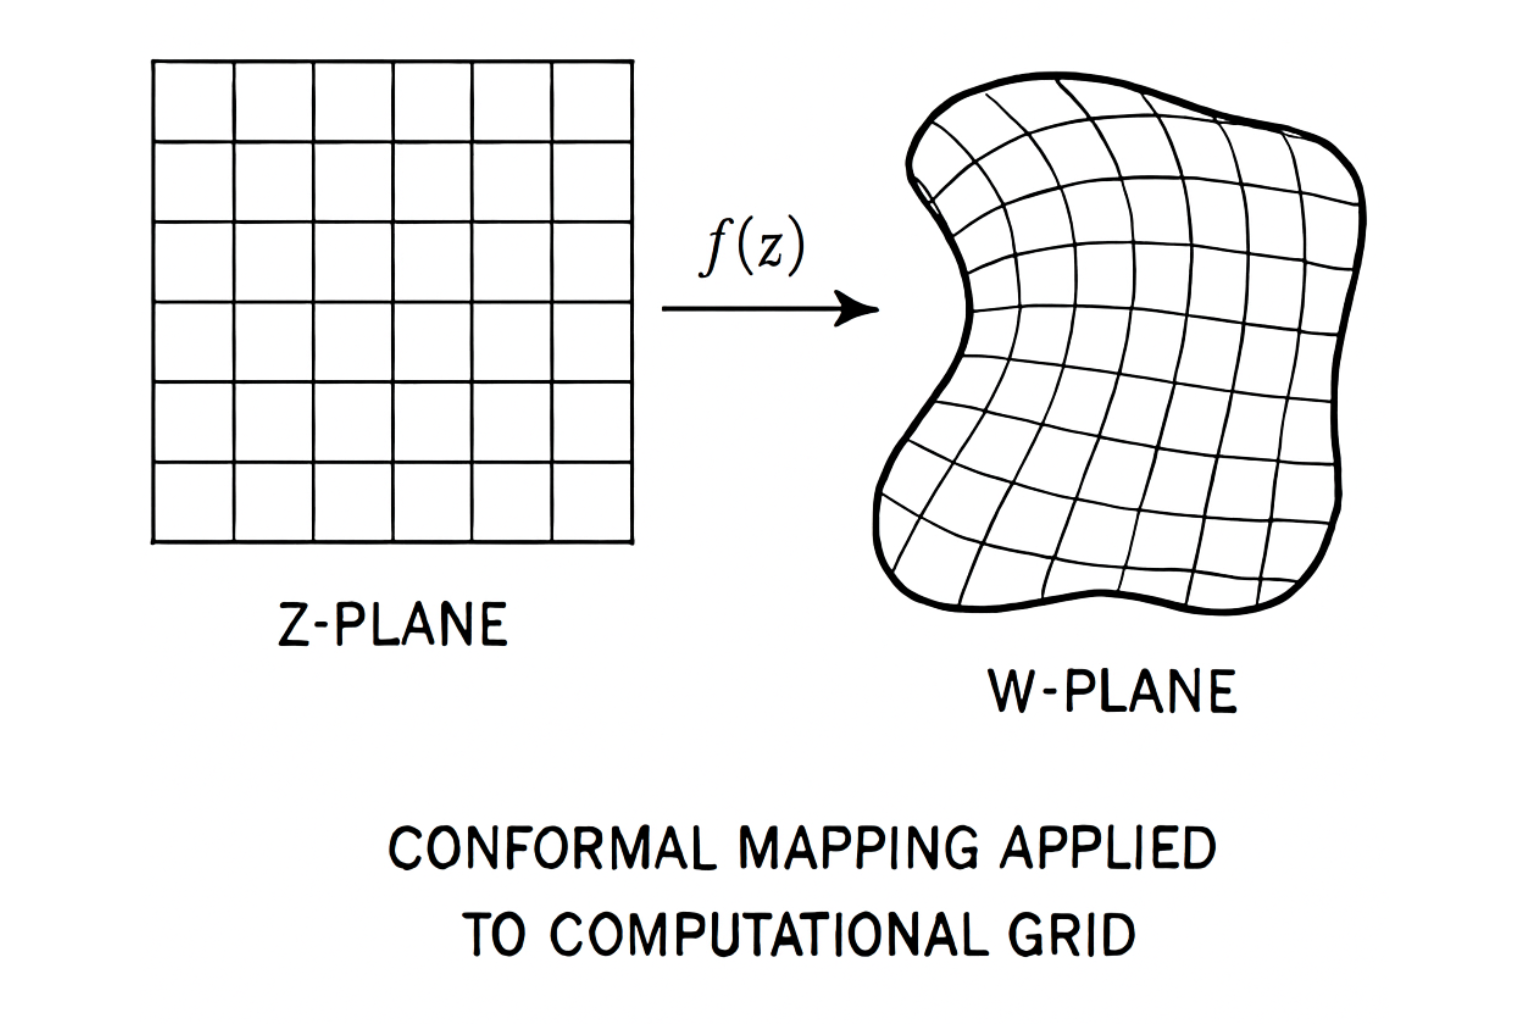
\includegraphics[width=0.8\textwidth]{Images/app-1-boundary-fitted orthogonal grids.png}
\caption{Boundary-Fitted Orthogonal Grid Generation Using Conformal Mapping}
\end{figure}

\begin{center}\rule{0.5\linewidth}{0.5pt}\end{center}

\newpage
\section{Conclusion}\label{conclusion-1}

Conformal mapping, rooted in the fundamental \textbf{Riemann Mapping
Theorem}, provides an elegant and powerful mathematical framework for
solving two-dimensional boundary value problems. The
\textbf{Schwarz-Christoffel Transformation} is the explicit,
constructive tool within this framework, allowing for the conformal
mapping of the upper half-plane onto any simple polygonal region.

While the resulting SC integral is often complex, involving special
functions like elliptic integrals, the formula's existence and structure
provide a direct link between the geometry of the target polygon (via
its exterior angles \(\alpha_k \pi\)) and the parameters of the mapping
(the pre-images \(x_k\)). The practical utility of the SC transformation
is demonstrated across diverse fields, from calculating lift on airfoils
in \textbf{aerodynamics} to solving for potential fields in
\textbf{electrostatics} and generating high-quality computational grids.

The interplay between theory and computation continues to drive
innovation in this field. The ongoing development of robust numerical
algorithms to solve the parameter problem and evaluate the resulting
elliptic integrals ensures that the Schwarz-Christoffel transformation
will continue to be a vital technique for modeling and solving
real-world problems. The success of the Schwarz-Christoffel
transformation is a powerful example of how pure mathematical theory can
yield highly practical and indispensable tools for solving real-world
problems. The continued research into numerical methods for the SC
integral, particularly for complex and multiply-connected domains,
ensures that this classical result will remain at the forefront of
computational science for decades to come.

\begin{center}\rule{0.5\linewidth}{0.5pt}\end{center}

\newpage
\section*{List of Important Symbols}
\addcontentsline{toc}{section}{List of Important Symbols}

\begin{itemize}
\item $z = x + iy$ - Complex variable in the source plane
\item $w = u + iv$ - Complex variable in the target plane
\item $f(z)$ or $w = f(z)$ - Conformal mapping function
\item $f'(z)$ or $\frac{dw}{dz}$ - Derivative of the mapping function
\item $\mathbb{C}$ - The complex plane
\item UHP - Upper half-plane, $\{z \in \mathbb{C} : \text{Im}(z) > 0\}$
\item $u(x, y)$, $v(x, y)$ - Real and imaginary parts of analytic function $f(z) = u + iv$
\item $\nabla^2 u$ - Laplacian operator
\item $n$ - Number of vertices of the polygon
\item $w_k$ - The $k$-th vertex of the polygon in the $w$-plane
\item $x_k$ - Pre-image of vertex $w_k$ on the real axis in the $z$-plane
\item $\theta_k$ - Interior angle at vertex $w_k$
\item $\alpha_k$ - Exterior angle parameter, where $\alpha_k = 1 - \frac{\theta_k}{\pi}$
\item $A$, $B$ - Complex constants in SC formula (scale, rotation, translation)
\end{itemize}

\section*{References}
\addcontentsline{toc}{section}{References}

\begin{itemize}
\item \textbf{Driscoll, T. A., \& Trefethen, L. N.} (2002). \textit{Numerical Conformal Mapping: Domain Decomposition and the Mapping of Quadrilaterals}. World Scientific Publishing.
\end{itemize}


\begin{center}\rule{0.5\linewidth}{0.5pt}\end{center}

\end{document}
